\section{Implementation mismatch}\label{sec:mismatch}

\subsection{Realised interconnection}
In an implementation the actuator realises the force $n\dot z$ with gain error,
delay $d_a\ge0$, zero-order hold and backlash.
The virtual oscillator receives a measured velocity with gain error, noise,
sensor delay $d_y\ge0$ and sampling.
Its stiffness $\omega_z^2$ is either nominal ($\omega_z=1$) or retuned.
Collecting static gain errors as $\eta_q,\eta_z$, the realised loop has the form
\begin{equation}\label{eq:realised}
\begin{aligned}
  \ddot q+q&=(n+\eta_q+c+w)\,[\dot z]_a+f_q,\\
  \ddot z+\omega_z^2z&=-(n+\eta_z+c-w)\,[\dot q]_y+f_z,
\end{aligned}
\end{equation}
where $[\cdot]_a,[\cdot]_y$ denote the actuator and sensor channels (delay, hold,
sampling), $c$ and $w$ are the common and antisymmetric coupling \emph{control}
actions of \cref{sec:control}, and $f_q,f_z$ collect bounded unmodelled forces
and noise.
As in~\citet{juchem2027restoring} we split the gain errors into a common and an
antisymmetric part,
\begin{equation}\label{eq:eta-split}
  \eta_c:=\tfrac12(\eta_q+\eta_z),\qquad \eta_w:=\tfrac12(\eta_q-\eta_z).
\end{equation}
With ideal channels, \eqref{eq:Hdot} gives the power balance
$\dot H=2(w+\eta_w)\dot q\dot z+(1-\omega_z^2)z\dot z+\dot qf_q+\dot zf_z$.
The antisymmetric part $w+\eta_w$ performs net work; the common part $c+\eta_c$
is power-neutral and only redistributes energy between the modes,
cf.~\eqref{eq:common-amp}.
The analysis below shows that delay and sampling, not static gain errors, are
the dangerous mechanisms; this matches the ablation in~\citet[Table~I]{juchem2027restoring}.

\subsection{Loop delay: exact spectral analysis}\label{sec:delay}
Consider \eqref{eq:realised} with ideal gains ($\eta=c=w=0$, $\omega_z=1$,
$f=0$) and pure delays, $[\dot z]_a=\dot z(t-d_a)$ and
$[\dot q]_y=\dot q(t-d_y)$.
The characteristic function depends only on the loop delay $d:=d_a+d_y$:
\begin{equation}\label{eq:quasi}
  \Delta(s;d)=(s^2+1)^2+n^2s^2e^{-sd}
  =F_+(s;d)\,F_-(s;d),
\end{equation}
with $F_\pm(s;d):=s^2+1\mp\ii ns\,e^{-sd/2}$.
Both factors are quasi-polynomials of \emph{retarded} type: the delayed term has
lower degree than the delay-free term.

\begin{theorem}[Delay destabilises the interconnection]\label{thm:delay}
Let $n>0$ and $d>0$. Then:
\begin{enumerate}
\item[(a)] $\Delta(\cdot;d)$ has a root on $\ii\RR$ only if $d\in\mathcal
  D_+\cup\mathcal D_-$, with $\mathcal D_\pm:=\{2\pi k/\Opm:k\in\NN\}$.
  The crossing roots are simple and lie at $\pm\ii\Op$ for $d\in\mathcal D_+$
  and at $\pm\ii\Om$ for $d\in\mathcal D_-$.
\item[(b)] Crossings at $\pm\ii\Op$ are always from left to right and crossings
  at $\pm\ii\Om$ always from right to left as $d$ increases.
\item[(c)] For $d\notin\mathcal D_+\cup\mathcal D_-$ the number of roots in
  $\Real s>0$, counted with multiplicity, is
  \begin{equation}\label{eq:Nd}
    N(d)=2\Big(1+\Big\lfloor\frac{d\Op}{2\pi}\Big\rfloor-\Big\lfloor\frac{d\Om}{2\pi}\Big\rfloor\Big)\ \ge\ 2.
  \end{equation}
  In particular, the interconnection is exponentially unstable for \emph{every}
  $d>0$.
\item[(d)] As $d\downarrow0$, the roots emanating from $\pm\ii\Op$ and
  $\pm\ii\Om$ satisfy
  \begin{equation}\label{eq:delay-rates}
    \Real s_\pm(d)=\pm\alpha_\pm(d)+O(d^2),\qquad
    \alpha_\pm(d):=\frac{n\Opm^2}{2S}\,d.
  \end{equation}
\end{enumerate}
\end{theorem}

The proof (\cref{app:delay}) is a direct crossing analysis in the spirit
of~\citet{cooke1986zeroes} and~\citet{walton1987direct}.
Two structural facts make it closed-form.
First, $|\omega^2-1|=n|\omega|$ has only the solutions $|\omega|=\Opm$, so the
imaginary-axis crossings can occur only at the nominal modal frequencies.
Second, the crossing direction is $\operatorname{sign}\Real\frac{\dd s}{\dd d}=\operatorname{sign}(\omega^2-1)$,
independent of $d$.
Because $\Op>\Om$, destabilising crossings occur more often than stabilising
ones, so stability is never recovered.
In particular, the system has no delay windows of the kind that make the delayed
resonator work~\citep{olgac1994novel}.
\Cref{fig:delay}(a) compares \eqref{eq:Nd} with the rightmost roots computed by
spectral collocation of the infinitesimal generator~\citep{breda2005pseudospectral}
followed by Newton refinement; the two agree for all $d\in(0,40]$\,s.

\begin{remark}[On truncating the spectrum]\label{rem:rightmost}
A retarded quasi-polynomial has finitely many roots in every half-plane
$\Real s>\beta$, and its root chains satisfy $\Real s\to-\infty$ as
$|s|\to\infty$~\citep{hale1993introduction,michiels2014stability}.
Stability is therefore decided by finitely many rightmost roots.
This justifies looking at a few poles only, but it does not say \emph{which} or
\emph{how many}.
Truncating with a Pad\'e approximant and applying the Routh--Hurwitz test only
approximates this.
The crossing argument above is exact and needs no truncation.
Routh-type arrays enter the exact methods only to locate the crossing
frequencies~\citep{walton1987direct,olgac2002exact}, and here those frequencies
are known in closed form.
\end{remark}

\begin{figure*}[t]
  \centering
  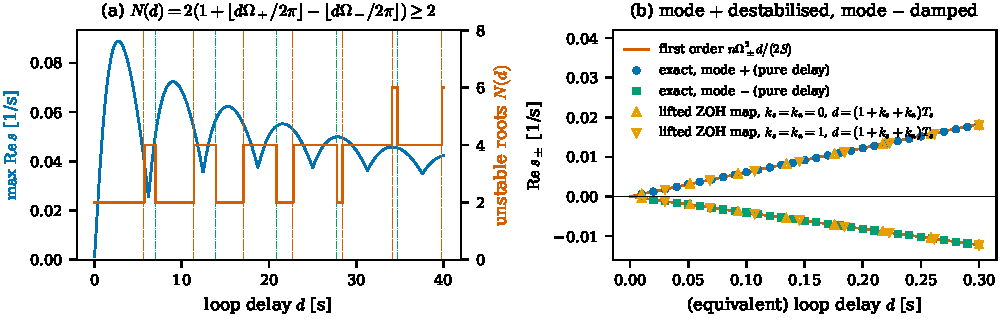
\includegraphics[width=\textwidth]{fig_delay.pdf}
  \caption{(a) Spectral abscissa of \eqref{eq:quasi} for $(11,9)$ and the
  closed-form count \eqref{eq:Nd}; dashed (dotted) lines mark destabilising
  (stabilising) crossing delays $\mathcal D_+$ ($\mathcal D_-$).
  (b) Small-delay regime: exact real parts of the $\pm$ modes for pure loop delay
  and for the lifted zero-order-hold map of \cref{prop:zoh} plotted against the
  equivalent loop delay, together with the first-order rates
  \eqref{eq:delay-rates}.}
  \label{fig:delay}
\end{figure*}

The first-order rates explain the observations of~\citet{juchem2027restoring}
mechanistically.

\begin{corollary}[Modal signature of a small delay]\label{cor:delay-modal}
Averaged over the fast phases, a small loop delay $d$ acts on the modal
amplitudes as $\avg{\dot A_+}=\alpha_+A_+$ and $\avg{\dot A_-}=-\alpha_-A_-$.
Hence
\begin{align}
  \avg{\dot\eA}&=\alpha_\Sigma:=\alpha_++\alpha_-\nonumber\\
  &=\frac{n(S^2-2)}{2S}\,d>0,\label{eq:alpha-sigma}\\
  \avg{\dot H}&=2H\big(\alpha_+a-\alpha_-(1-a)\big),\label{eq:H-delay}
\end{align}
with $a$ the energy share \eqref{eq:share}.
A delay therefore pumps energy into the fast mode and drains the slow mode.
It produces both energy drift and modal imbalance, and the imbalance grows at a
\emph{state-independent} rate.
\end{corollary}
\begin{proof}
Use $\dot z(t-d_a)=\dot z-d_a\ddot z+O(d_a^2)$ and the same expansion for $\dot q$,
so that, to first order, $\Delta_1=nd_a(z+n\dot q)$ and
$\Delta_2=nd_y(-q+n\dot z)$ in \cref{lem:perturbed}.
Average \eqref{eq:Adot} over the torus using \cref{lem:modal}, e.g.\
$\avg{X_+z}=A_+^2/2$ and $\avg{X_+\dot q}=\Op A_+^2/2$, together with
$1+n\Op=\Op^2$ and $1-n\Om=\Om^2$.
This yields $\avg{\tfrac{\dd}{\dd t}\tfrac{A_\pm^2}{2}}=\pm\alpha_\pm A_\pm^2$, and
\eqref{eq:alpha-sigma}--\eqref{eq:H-delay} follow from \eqref{eq:errors} and
\cref{lem:modal}(3).
\end{proof}

\subsection{Zero-order hold}\label{sec:zoh}
\begin{assumption}[Sampled implementation]\label{ass:sampled}
The host velocity is sampled at $t_k=kT_s$ with a delay of $k_y\in\NN_0$
samples.
The virtual oscillator is integrated exactly over $[t_k,t_{k+1})$ with its
coupling input held constant.
The actuator command $n\dot z(t_k)$ is held constant over $[t_k,t_{k+1})$ and
applied with a delay of $k_a\in\NN_0$ samples.
\end{assumption}

Under \cref{ass:sampled} the loop is exactly a finite-dimensional linear
discrete-time system.
For $k_y=k_a=0$ it is $x_{k+1}=\Phi(T_s)x_k$ with
$\Phi(T_s)=e^{A_0T_s}+\int_0^{T_s}e^{A_0\vartheta}\dd\vartheta\,G$, where
$A_0$ is the uncoupled part and $G=A_c-A_0$ the coupling; for $k_y,k_a>0$ the
map is lifted with buffer states.

\begin{proposition}[ZOH as an equivalent delay]\label{prop:zoh}
Under \cref{ass:sampled} with $k_y=k_a=0$,
\begin{equation}\label{eq:zoh-gen}
  \tfrac{1}{T_s}\log\Phi(T_s)=A_c-\tfrac{T_s}{2}\,GA_c+O(T_s^2).
\end{equation}
The right-hand side coincides, to first order, with the generator of the
continuous loop with delay $T_s/2$ in each channel.
Consequently the eigenvalues of $\Phi(T_s)$ satisfy
$T_s^{-1}\log|\lambda_\pm|=\pm\alpha_\pm(\deq)+O(T_s^2)$ with $\deq=T_s$, and
with sample delays $\deq=(1+k_y+k_a)T_s$.
In particular, the spectral radius of the sampled loop exceeds one for all
sufficiently small $T_s>0$.
\end{proposition}
\begin{proof}
Expanding, $\Phi(T_s)=I+T_sA_c+\tfrac{T_s^2}{2}(A_0^2+A_0G)+O(T_s^3)$.
Since $A_c^2-GA_c=A_0^2+A_0G$, this equals
$\exp\big(T_sA_c-\tfrac{T_s^2}{2}GA_c\big)+O(T_s^3)$; the
Baker--Campbell--Hausdorff correction is $O(T_s^3)$.
A delay $\delta$ in both channels gives, to first order,
$\dot x=A_0x+G(x-\delta\dot x)=A_cx-\delta GA_cx$, so $\delta=T_s/2$ and the loop
delay is $T_s$.
Each sample of buffering adds $T_s$ to its channel.
The rates follow from \cref{thm:delay}(d), since the first-order eigenvalue shift
depends only on $d_a+d_y$.
\end{proof}

\Cref{fig:delay}(b) confirms \eqref{eq:zoh-gen}: the lifted ZOH map with
$k_y=k_a\in\{0,1\}$ falls on the pure-delay curve when plotted against $\deq$.
For the example of~\citet{juchem2027restoring} ($T_s=0.03$\,s and one-sample
sensor and actuator delays), $\deq=0.09$\,s and the fast mode grows at
$\alpha_+=5.5\times10^{-3}$\,s$^{-1}$.
\gap{ZOH instability for all $T_s$}{\cref{prop:zoh} is first order. Numerically
$\rho(\Phi(T_s))>1$ for all $T_s\in(0,3]$\,s (code/vms/zoh.py). The
characteristic polynomial of $\Phi$ is an explicit quartic in $\lambda$ with
trigonometric coefficients in $T_s$, so a symbolic Jury/Schur--Cohn test should
settle the claim for all $T_s>0$.}

\begin{remark}[Software integrator]
\Cref{ass:sampled} assumes exact (or symplectic) integration of the virtual
oscillator.
A forward-Euler integrator adds an anti-damping of order $T_s/2$ to the virtual
oscillator, which adds to $\alpha_\pm$.
Geometric integrators~\citep{hairer2006geometric} and discrete port-Hamiltonian
models~\citep{stramigioli2005sampled} avoid this.
\end{remark}

\subsection{Static mismatch and retuning authority}\label{sec:authority}
Static gain errors behave very differently from delays.

\begin{proposition}[First-order effect of static mismatch]\label{prop:static}
For constant $\eta_c,\eta_w$ and $\varepsilon:=\omega_z^2-1$, the first-order
averaged effect on $(H,\eA)$ is zero.
The effect on the relative phase is
\begin{equation}\label{eq:psi-static}
  \avg{\dot\psi}=\beta_\psi\,\eta_c-b_\psi\,\varepsilon,\qquad
  \beta_\psi:=\frac{2\sqrt{\tau\sigma}}{S},\quad b_\psi:=\frac{\tau-\sigma}{2S}.
\end{equation}
\end{proposition}
\begin{proof}
For $\eta_w$: $\Delta_1=\eta_w\dot z$, $\Delta_2=\eta_w\dot q$, and by
\cref{lem:modal} all terms of \eqref{eq:Adot} are products of
harmonics with non-zero frequencies $2\Op$, $2\Om$, $\Op-\Om$.
For $\eta_c$: \eqref{eq:common-amp} is proportional to $\sin\varphi$.
For $\varepsilon$: $\Delta_2=-\varepsilon z$ gives harmonics in $2\Opm$ and
$\Op\pm\Om$.
None of these frequencies vanishes, so every average is zero.
For the phases, \eqref{eq:thdot} gives
$\avg{\dot\theta_\pm}-\Opm=\pm\eta_c\Opm/S+\varepsilon/(2S)$, i.e.\ the
eigenvalue sensitivities $\partial\Opm/\partial n=\pm\Opm/S$ and
$\partial\Opm/\partial\varepsilon=1/(2S)$.
With \eqref{eq:n-design}, $\sigma\Op+\tau\Om=2\sqrt{\tau\sigma}$, which gives
\eqref{eq:psi-static}.
\end{proof}

Static gain errors therefore only detune the resonance, and the relative phase
drifts at a constant rate.
This is consistent with the small energy and amplitude errors that gain errors
alone produce in~\citet[Table~I]{juchem2027restoring}.
To restore the ratio, \citet{juchem2027restoring} retunes the virtual stiffness.
The next result shows why this is a poor actuator.

\begin{proposition}[Retuning authority]\label{prop:authority}
For constant couplings $N_q=n+a$, $N_z=n+b$ and virtual stiffness $\omega_z^2$,
the modal frequencies are the positive roots of
$\omega^4-(1+\omega_z^2+\kappa)\omega^2+\omega_z^2=0$, with $\kappa:=N_qN_z$.
The ratio $r=\omega_+/\omega_-$ satisfies
\begin{equation}\label{eq:ratio}
  r+\frac1r=\frac{1+\omega_z^2+\kappa}{\omega_z}.
\end{equation}
Consequently, with $n$ from \eqref{eq:n-design}:
\begin{enumerate}
\item[(a)] Retuning $\omega_z$ alone attains $r=\tau/\sigma$ if and only if
  $\kappa\le n^2+n^4/4$.
  For a common relative error $\kappa\approx n^2(1+2\delta)$ this means
  $\delta\le n^2/8$.
  Moreover $\partial r/\partial\omega_z=-n\Op^2/S$ at the nominal point, and
  $\partial r/\partial\omega_z=0$ at $\omega_z=\sqrt{1+\kappa}$.
\item[(b)] Retuning a common coupling trim $c$ ($a=b=c$, $\omega_z=1$) attains
  $r=\tau/\sigma$ for every $\kappa>0$, with $\partial r/\partial c=2\Op^2/S$ at
  the nominal point.
\end{enumerate}
\end{proposition}
\begin{proof}
The characteristic polynomial of \eqref{eq:realised} with constant parameters is
$(s^2+1)(s^2+\omega_z^2)+\kappa s^2$.
Vieta's formulas give $\omega_+^2+\omega_-^2=1+\omega_z^2+\kappa$ and
$\omega_+\omega_-=\omega_z$, hence \eqref{eq:ratio}.
For fixed $\kappa$ the right-hand side is minimal at $\omega_z=\sqrt{1+\kappa}$,
with value $2\sqrt{1+\kappa}$.
The target value $\tau/\sigma+\sigma/\tau=2+n^2$ is attainable iff
$2\sqrt{1+\kappa}\le2+n^2$, i.e.\ $\kappa\le n^2+n^4/4$.
The derivatives follow by differentiating \eqref{eq:ratio}, using
$1-r^{-2}=nS/\Op^2$ at the nominal point.
For (b), \eqref{eq:ratio} with $\omega_z=1$ reads $r+1/r=2+\kappa$, which is
increasing in $\kappa$; any target $r>1$ is attained by $\kappa=n^2$.
\end{proof}

For $(11,9)$, $n^2/8=0.5\%$: a net positive common gain error above half a
percent makes the frequency target of~\citet{juchem2027restoring}
\emph{unreachable}.
Even below that threshold, the sensitivity collapses about $n^2/2\approx2\%$ away
from $\omega_z=1$ (\cref{fig:retuning}).
The example of~\citet{juchem2027restoring} has
$\kappa\approx(1.065)(0.97)\,n^2$, i.e.\ $\kappa-n^2\approx0.033\,n^2$
(ignoring backlash), well above $n^4/4\approx0.01\,n^2$.
The frequency loop there therefore cannot converge and hunts
(\cref{sec:sim}).
The common coupling, by contrast, has authority larger by a factor $2/n\approx10$
and a monotone characteristic, and it is the actuator used in \cref{sec:control}.

\begin{figure*}[t]
  \centering
  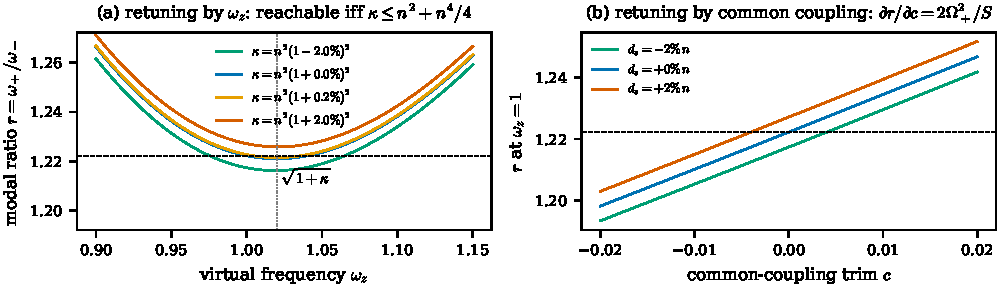
\includegraphics[width=\textwidth]{fig_retuning.pdf}
  \caption{Retuning the modal ratio for $(11,9)$. (a) By the virtual frequency
  $\omega_z$: the target (dashed) is reachable only if
  $\kappa\le n^2+n^4/4$, and the sensitivity vanishes at
  $\omega_z=\sqrt{1+\kappa}$. (b) By a common coupling trim $c$ at $\omega_z=1$:
  monotone, with slope $2\Op^2/S$.}
  \label{fig:retuning}
\end{figure*}
